\chapter{Controlling The Motors}

%Keywords: PWM, Encoder, H-bridge, direction control, , position controller, speed controller, straight forward controller
%duty cycle, measurements and tests, pwm frequency, h-bridge limitations
%Figures: PWM, H-bridge output (measurement), tacho (theory + measurement), schematic (section cut), direction table, 




\section {The DC-motor}


\subsection{DC-motor}
The DC-motor is a essential part of the robot. The motors used in this project is the Faulhaber 2233012s which is a 12 Volt armature motor.  To succeed the tasks given in the assignment is it very importent to gain control over the motor by understand the datasheet that describes the motor. The motors dose not only supply the robot with driving force but is also the steering part of the robot.

\subsection{Gears}
To give the robot more torque a gear system has been implemented in the motors. The cost of high torque through a gearsystem is a reduction in rotational speed. The gearing factor that is used is $\frac{1}{17.2}$ which means that the output shaft only turns one cycle every times the motor itself have turned 17.2 cycles. The gear system do have some disadvantages by giving the motor nonlinearity like backlash and deadlocks. 
\subsection{Transferfunction for DC-motor}
In assignment 1 from the control theory course we calculated a transfer function for at DC-motor. By using this knowledge and theory we a able to calculate a transfer function for the DC-motor used in this project.
The transfer function for the DC-motor is needed for making simulations of the hole system later on.\\
All motor data is fund in the datasheet and the weight of the robot is fund by weighting the robot on a digital precision scales and is fund to be 1400 g or 1.4 Kg. \\

The general transfer function:

\begin{equation}
G(s)=\frac{\theta_m(s)}{E_a(s)} \Rightarrow \frac{\frac{k_t}{R_a J_a}}{s+\frac{1}{J_a}(D_a + \frac{K_bK_t}{R_a})}
\end{equation}
  
 The transfer function for the robot: 

\begin{equation}
G(s)=\frac{\omega(s)}{E_a(s)}=\frac{\frac{1633}{23.43}}{s\frac{1}{23.43} +1} = \frac{69,69}{0,04268+1}
\end{equation}  

Where $0.04268$ is the time constant. \\
The step respons on the DC-motor looks like this:

\begin{figure}[!h]
	\centering
	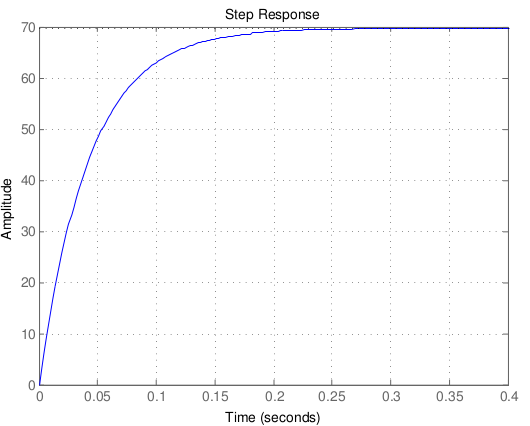
\includegraphics[width=0.6\textwidth]{resources/motor_transfer_function.png}
	\caption{Step respons for DC-motor}
	\label{fig:2}
\end{figure}


\section{Microcontroller} 
The MCU (Microcontroller) is the first part of the link between the sensor input and the DC-motor. In the MCU a translation is made so that the DC-motor can be controlled using simple I2C (Two way communication) commands from the sensor device. A controller is also implemented in the MCU so that the robot is able to run straight without any further instructions from the sensor device.\\

The MCU decodes the command form the sensor devise and then extracts informations about direction and speed. These informations is then sends down to the H-bridge and ends as Voltage in the DC-motor.

\subsection{The MCU}
The MUC used in the robot is an Atmel ATxmega192c3 a 8bit low-power microcontroller with 192kbyte flash memory running a clock frequency at 32 MHz. The choice of this MCU is based on the its speed performance and its high level of functionality features. The first MCU used in the robot was a Atmel Atmega 32 but after a brief discussion in the group and with the project supervisor we decided to change the MUC because we previously worked with the Atmega32 and wanted to explore more recent technologies and the opportunity to work with the SMD (surface mounted device) method. 

\subsection{Programming}
The MUC is programed using Atmels studio 6.1 and the program language used is C. The ASF(Atmel Software Framework) libraries has be used in great extent. For more informations here about visit:\\  www.atmel.com/tools/avrsoftwareframework.aspx \\
The source code for the MCU can be found in the appendix. 

\section{H-bridge}

The H-bridge receive three line per motor from the MCU The first line controls the speed with a PWM signal and the to other lines control the rotational direction of the motor.


\newpage

\subsection{PWM Pulse-width modulation}

PWM (Pules-width modulation) is a method frequently used in electronics. The signals intensity it controlled by changing the duty cycle for a square wave signal with a predefined frequency. The controllable range is from 0$\% $ to 100$\%$ 
The frequency of the square has been chosen to be 20kHz so that is it over the human hearing range. 
\\
The figures below shows how a 25$\%$ and a 50$\%$  PWM looks between the MCU and the H-bridge. The duty cycle output of the MCU is about 15 $\%$ and 82$\%$ The reason for that is that the controller in the MCH manipulates the PWM, more about this in the Feedback and Control Loop section.

  \begin{figure}[!h]
	\centering
	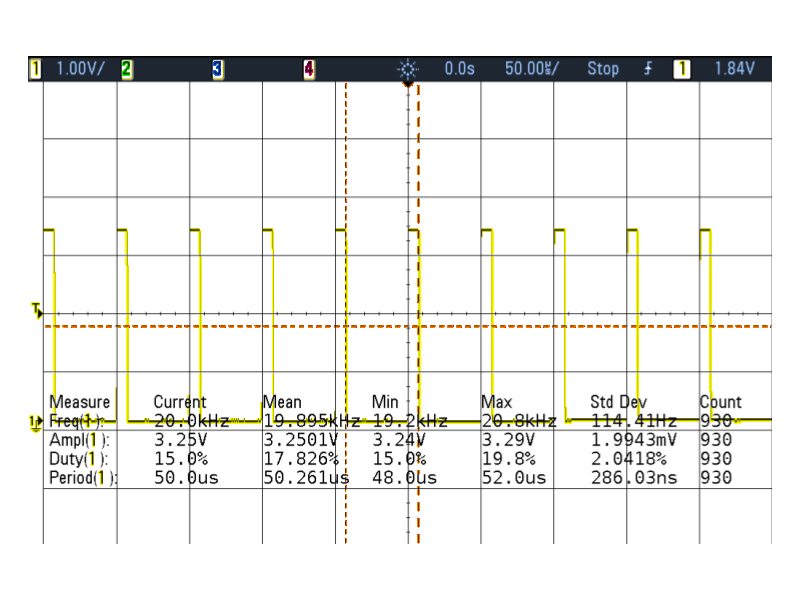
\includegraphics[width=0.55\textwidth]{resources/Scop/PWM_motot_right_PWMin25.png}
	\caption{PWM with input at 25$\%$}
	\label{fig:1}
\end{figure}

  \begin{figure}[!h]
	\centering
	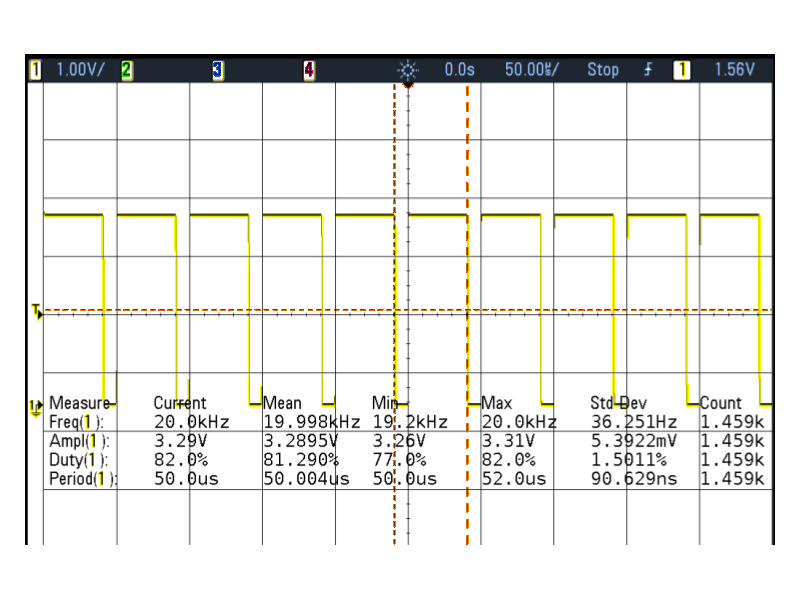
\includegraphics[width=0.55\textwidth]{resources/Scop/PWM_motot_right_PWMin50.png}
	\caption{PWM with input at 50$\%$}
	\label{fig:2}
\end{figure}

\newpage
\subsection{Direction control} 
To control the direction of the motor the H-bridge receives two lines A1 and A2 these two lines dictates the rotational direction of the DC-motor.

  \begin{figure}[!h!]
	\centering
	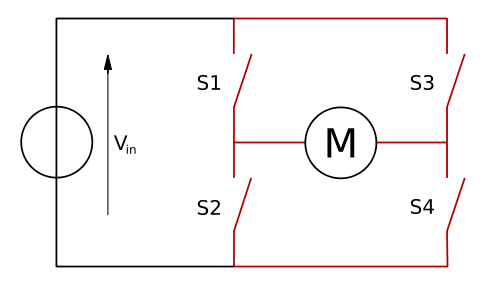
\includegraphics[width=0.6\textwidth]{H-bridge_diagram.png}
	\caption{H-bridge}
	\label{fig:3}
\end{figure}
When line A1 is high and line A2 is low the corresponding switches S1 and S4 is closed so that the current is running in one direction. when A1 is low and A2 is high the current is running the other way and the motor it turning the other way around. \\

 below is a truth table that describes the functionality of the H-bridge. The EN pin is the PWM input.  

  \begin{figure}[!h!]
	\centering
	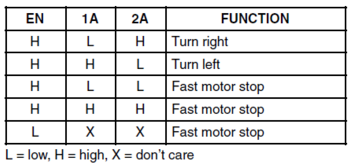
\includegraphics[width=0.6\textwidth]{H-bridge_table.png}
	\caption{H-bridge truth table}
	\label{fig:4}
\end{figure}

\newpage
\section{Encoders}
  The DC-motor includes two encoder outputs which is used to determine position, velocity and direction of the DC-motor.
  Each encoder outputs 15 pulses per round and after the gear is the resolution $15 \cdot 17.2 = 258$ pulses per round.
  The two encoder signals is phase shifted at about $\ang{90}$ and that gives us the opportunity to determine the rotational direction of the motor by looking at one encoder signal and then check if the other one it high or low. This method is illustrated below in figure 3.6.
   
  \begin{figure}[!h!]
	\centering
	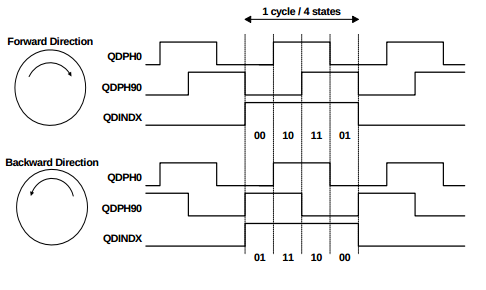
\includegraphics[width=0.7\textwidth]{resources/encoder_atmel.png}
	\caption{Encoder illustration from atmel Application Note AVR 1600 aboute Quadrature Decoder}
	\label{fig:5}
\end{figure}

On figure 3.7 we see the actual encoder output from the robot. The phase is about $\ang{100}$ between the two encoders.
  \begin{figure}[!h!]
	\centering
	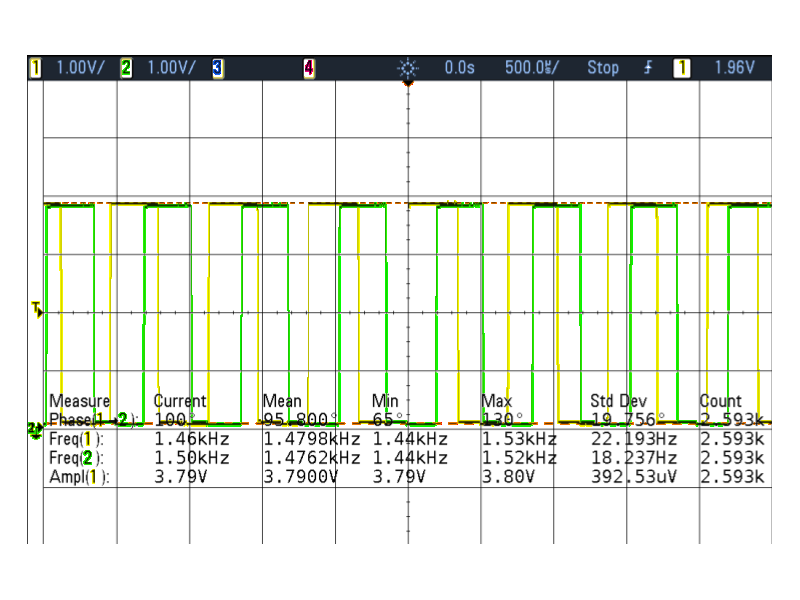
\includegraphics[width=0.8\textwidth]{resources/Scop/encoder.png}
	\caption{Encoder output from Motor to MCU}
	\label{fig:6}
\end{figure}
%-----------------------------------------------------_SKAL RETTES _-----------------------------------------
The velocity is found by sampling the encoder pulses over a time period of 10ms, by counting the pulses during this time and multiply it with a constant the velocity of the motor is given.
Also the position between the two motors can be find by using two encoders on each motor. First we look at one motor encoder count and then match up the other motor so that the encoder count from the to motors fits, then we know the exact position of the robot. We use these method in the position controller.    
%skal rettes---------------------------------------------------------------------------------------------------
\newpage

\section{Feedback and Control Loop}
The control loop containing the motor,MCU and encoder can be described as a unity feedback loop.


  \begin{figure}[!h!]
	\centering
	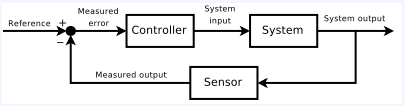
\includegraphics[width=0.8\textwidth]{resources/feedbackloop.png}
	\caption{Unity feedback loop}
	\label{fig:6}
\end{figure}





The MCU have three different stats with three different controllers so that it can adapt to the given situation during the track. The three states are:


\begin{itemize}
\item 1. Straight
\item 2. Position
\item 3. Speed
\end{itemize}

The selection of which current stat the MCU should be in is determiant by the raspberry pi(sensor system).

\subsection{Straight state}
This state is designed to make the robot go straight without any corrections from the sensor system.This it done by given both motors a reference speed and then aligning them after the outputs from the encoders by adjusting the speed to each motor. 


\subsection{Position state}


\subsection{Speed state}
This state is used when the robot follows the line by adjusting after instruction from the sensor system. A P-controller it used and the encoders have no influence on the control of the motor.
